\documentclass[10pt]{beamer}

%%%
% PREAMBLE FOR THIS DOC 
%%%
%https://tex.stackexchange.com/questions/68821/is-it-possible-to-create-a-latex-preamble-header
\usepackage{/Users/miw267/Repos/csci246_spring2025/slides/preambles/beamer_preamble_for_CSCI246}

\usetikzlibrary{matrix}


%%% TRY TO RESHOW TOC AT EACH SECTION START (with current section highlighted)
% Reference: https://tex.stackexchange.com/questions/280436/how-to-highlight-a-specific-section-in-beamer-toc
\newcommand\tocforsect[2]{%
  \begingroup
  \edef\safesection{\thesection}
  \setcounter{section}{#1}
  \tableofcontents[#2,currentsection]
  \setcounter{section}{\safesection}
  \endgroup
}


%%%% HERES HOW TO DO IT CORRECTLY
% FIRST IN .STY FILE, DO
%\usetheme[sectionpage=none]{metropolis}
% THEN AT EACH SECTION DO
%\begin{frame}{Outline}
%  \tableofcontents[currentsection]	
%\end{frame}



%\setbeamertemplate{navigation symbols}{}
%\setbeamertemplate{footline}[frame number]{}


%%%
% DOCUMENT
%%%

\begin{document}

%\maketitle

%% Title page frame
%\begin{frame}
%    \titlepage 
%\end{frame}




%
%\title{03/12/2025: Intro to Probability (Part 1): \\ \qquad \qquad \qquad Sample Space \& Events}
\title{03/12/2025: Intro to Probability (Part 1)}
\author{CSCI 246: Discrete Structures}
\date{Textbook reference: Sec 30, Scheinerman}

\begin{frame}
    \titlepage 
\end{frame}


\begin{frame}
\footnotesize 
\begin{mygreenbox}[title=Graded Quiz Pickup]
Quizzes are in the front of the room, grouped into four bins (A-G, H-L, M-R, S-Z) by last name. The quizzes are upside down with your last name on the back. Come find yours before, during, or after class.  Only turn the quiz over if it's yours.
\end{mygreenbox} 
\vfill 

\begin{myredbox}[title=Announcement: Friday 03/14 will be a review day]
\begin{enumerate}
	\item No reading assignment,  reading quiz, or problem quiz. 
	\item We review group exercises from binomial coefficients, inclusion/exclusion, and intro to probability 1.
	\item Time permitting, we will also have an open Q \& A.  Feel free to bring questions on any topic we've covered so far.
\end{enumerate}
\end{myredbox}

\vfill 


\begin{myyellowbox}[title=Today's Agenda]
\begin{itemize}
	\item Reading quiz (5 mins)
	\item Mini-lecture ($\approx$ 25 mins)
%	%
%	\begin{itemize}
%	\footnotesize 
%	\item Review induction 
%	\end{itemize}
%	%
	\item Group exercises ($\approx$ 15 mins)
\end{itemize}

%	Rationale for group exercises: we got shortchanged on time last couple days, and I already did a lot of lectures, so I want you to practice. Next problems quiz will cover relations and functions: Hamkins and 
%	
\end{myyellowbox}
\vfill 

\end{frame}

\begin{frame}[standout]
Feedback on Monday's Quiz
\end{frame}

\begin{frame}{Reading Quiz}
\footnotesize 
\begin{figure}[ht]
        \centering
        \includegraphics[width=.6\textwidth]{images/reading_quiz_scores}
   		 \caption{Median Score = 7/8 (87.5\%)}
\end{figure}
\vfill 
\textbf{Rubric.}  	
\begin{enumerate}
\item  6 points. One point for each sign.
\item 1 point.  
\item 1 point. 
\end{enumerate}
\end{frame}	



\begin{frame}

\begin{mygreenbox}[title= Some nice creative thinking in answering Question \#2]
\footnotesize 
\textbf{Question.}  (True or False.) Consider the length-$k$ lists whose elements are chosen from the set $\set{1,2,\hdots, n}$.  The number of lists which use all of the elements in $\set{1,2,\hdots, n}$ at least once is $n^k$. \\

\textbf{Student answers.}
\begin{itemize}
\item False.  Let $n=3$, so we're choosing elements from $\set{1,2,3}$.  Let $k=3$. Then the lists which contain all the elements are 
\[ \bigg\{ (1,2,3), (1,3,2), (2,3,1), (2,1,3), (3,2,1), (3,1,2) \bigg\}.\] 	
There are 6 items in this list, and $6 \neq n^k = 3^3= 27$.
\item False.  By the question $k<n$ is valid, and if $k<n$ then no lists can contain all elements.
\end{itemize}

\end{mygreenbox}

%\begin{mygreenbox}[title= Some nice answers to Question \#3]
%\footnotesize 
%\textbf{Question.}  (True or False.) Consider the length-$n$ lists whose elements are chosen from the set $\set{1,2,\hdots,n}$ without repetition. A list is called a \textit{derangement} if the number $j$ does not occupy position $j$ in the list for any $j=1,2,\hdots,n$.  The number of derangements is $n!$. 
%\vfill 
%\textbf{Answer.} If $n=0$, we're choosing elements from the $\emptyset$.  The claim is that the number of derangements would be $n!=0!=1$, which is false. 
%\end{mygreenbox}

\end{frame}



\begin{frame}[standout]
Reading quiz
\end{frame}

\begin{frame}

\begin{mygreenbox}[title=\text{Reading Quiz}]
A \textit{hand} of poker is a five-element subset of the standard deck of 52 cards.   Assuming that the deck is well-shuffled, what is the probability of drawing the hand $6 \clubsuit -K \heartsuit - 3 \diamondsuit - A \spadesuit - 7 \clubsuit$?
\end{mygreenbox}
	
\end{frame}


\begin{frame}[standout]
Additional thought on inclusion/exclusion
\end{frame}

\begin{frame}
\footnotesize 
\begin{myredbox}[title=Definition]
A \textbf{derangement} is a permutation of the elements of a set in which no element appears in its original position.	 That is, a derangement is a list of length $n$ using the elements of $\set{1,\hdots, n}$ such that the number $j$ does not occupy position $j$ of the list for any $j=1,\hdots n$.
\end{myredbox}
\vfill 
\begin{mygreenbox}[title=\text{Proposition (Scheinerman pp.114)}]
\[\# \text{derangements} = n! \sum_{k=0}^n \frac{(-1)^k}{k!} \]
\end{mygreenbox}
\vfill 
\begin{myyellowbox}[title=Poll]
Suppose that a professor gave a test to 4 students – A, B, C, and D – and wants to let them grade each other's tests. Of course, no student should grade their own test. How many ways could the professor hand the tests back to the students for grading, such that no student receives their own test back?
\end{myyellowbox}
	
	
\end{frame}

\begin{frame}{Solution}
\footnotesize 


\begin{myredbox}[title=Enumeration Solution]
 Out of 24 possible permutations (4!) for handing back the tests, there are only 9 derangements (shown in blue italics below). In every other permutation of this 4-member set, at least one student gets their own test back (shown in bold red).
 \begin{figure}
\includegraphics[width=.5\textwidth]{images/derangements.png}	
\end{figure}
\end{myredbox}
\vfill 
\pause 


\begin{mygreenbox}[title=Formulaic Solution]
\begin{align*}
\# \text{derangements} &= n! \sum_{k=0}^n \frac{(-1)^k}{k!} && \scripttext{(General formula)} \\
&= 4! \sum_{k=0}^4 \frac{(-1)^k}{k!} && \scripttext{(Substitute $n=4$)} \\
&= 4! \bigg(\frac{1}{0!} - \frac{1}{1!} + \frac{1}{2!} - \frac{1}{3!} + \frac{1}{4!} \bigg) && \scripttext{(Expand sum)}  \\
&= 4! - 4! + 4 \cdot 3 - 4 + 1 && \scripttext{(Distribute $4!$, simplify)} \\  
&= 12-4+1 = 9  
\end{align*}
\end{mygreenbox}


	

\end{frame}



\begin{frame}[standout]
Introduction to Probability: \\
Samples and Events
\end{frame}

\begin{frame}

\begin{myyellowbox}[title=Poll]
Imaging tossing two coins and observing whether 0, 1, 2 heads are obtained.  Will each of these events occur about 1/3 of the time?
\end{myyellowbox}

\pause 
\vfill 

\begin{figure}
\includegraphics[width=.8\textwidth]{images/coins_1.png}	
\end{figure}

Empirically, 1 head is obtained about twice as often as the other options. Why?  \pause  We'll clarify this matter in the next two slides.



%\begin{figure}
%\includegraphics[width=.8\textwidth]{images/coins_2.png}	
%\end{figure}
	
\end{frame}



\begin{frame}
\small 
\begin{mygreenbox}[title=Definition]
A (finite) \textbf{probability space} is a pair $(S,P)$ where $S$ is a finite, nonempty set and $P$ is a function $S \to \R$ such that $P(s) \geq 0$ for all $s \in S$ and 
\[ \sum_{s \in S} P(s) =1 \] 
\end{mygreenbox}
\vfill 
%	\begin{myredbox}[title=\text{Overview}]
%A \textbf{sample space} is the set of all possible outcomes of a random process or experiment. An \textbf{event} is a subset of the sample space.
%\end{myredbox}

\pause 
\vfill 

\begin{myredbox}[title=\text{Remark: What is a sample space?}]

A \textbf{sample space} is the set of all possible outcomes of a random process or experiment. \\

Scheinerman refers to $(S,P)$ as a \textit{sample space}.  However, most people  use \textit{sample space} to refer to $S$ alone.  (We will follow the latter convention.)
\end{myredbox}


\pause 
\vfill 

\begin{myyellowbox}[title=Example Of A Probability Space]

In the coin example, we can construct the probability space as 
\[S = \set{\texttt{HH}, \texttt{HT}, \texttt{TH}, \texttt{TT}} \]
and $P(s) = 1/4$ for all $s \in S$.
\end{myyellowbox}

\end{frame}

\begin{frame}
\small 
\begin{myredbox}[title=Overview]
An \textbf{event} is a subset of a sample space.  
\end{myredbox}
\vfill \pause
\begin{mygreenbox}[title=Definition]
Let $(S,P)$ be a probability space.  Then an \textbf{event} $E$ is a subset of $S$ (i.e. $E \subseteq S$).  The probability of an event $E$, denoted $P(E)$ is
\[ P(E) = \sum_{s \in E} P(s) \]
\end{mygreenbox}
\vfill \pause

\begin{myyellowbox}[title=Poll]
In the coin example, what is the event of observing one head?  What is its probability? \pause  The event of observing one head is $E = \set{\texttt{HT}, \texttt{TH}}$.  \pause The probability of the event is $P(E) = P(\set{\texttt{HT}}) + P(\set{\texttt{TH}}) = \frac{1}{4} + \frac{1}{4} = \half$. \pause 
	
\begin{figure}
\includegraphics[width=.8\textwidth]{images/coins_2.png}	
\end{figure}

\end{myyellowbox}


\end{frame}



\begin{frame}
\begin{mygreenbox}[title=Equally Likely Probability Formula]
If $(P,S)$ is a probability space in which all outcomes are equally likely and E is an event in $S$, then the probability of $E$ is
%
\begin{align*}
P(E) = \frac{|E|}{|S|} = \frac{\text{the number of outcomes in } E }{\text{the number of outcomes in } S}	
\end{align*}
\end{mygreenbox}
%\vfill 
%In the above, we have used the following notation
%\vfill 
%\begin{myredbox}[title=Notation]
%For any finite set $A$, $N(A)$ denotes the number of elements in $A$.
%\end{myredbox}

\end{frame}


\begin{frame}[standout]
Introduction to Probability: \\
Some Applications
\end{frame}


\begin{frame}
\footnotesize 
\begin{myredbox}[title=Background on cards]
An ordinary deck of cards contains 52 cards divided into four \textit{suits}.  The \textit{red suits} are 	diamonds ($\diamondsuit$) and hearts ($\heartsuit$), and the \textit{black suits} are clubs ($\clubsuit$) and spades ($\spadesuit$).  Each suit contains 13 cards of the following \textit{denominations}: 2, 3, 4, 5, 6, 7, 8, 9, 10, J (jack), Q (queen), K (king), and A (ace).  The cards J, Q, and K are called \textit{face cards}. 	
\end{myredbox}
\vfill 
\begin{myyellowbox}[title=Poll]
 Suppose we draw a card randomly from a shuffled deck.  (1)  What is the sample space of outcomes? (2) What is the event that the chosen card is a black face card. (3) What is the probability that the chosen card is a black face card?
\end{myyellowbox}
\pause 
\begin{mygreenbox}[title=Solution]
\begin{enumerate}
	\item The sample space $S$ are the 52 cards in the deck.
	\item \pause 
	\[E = \set{ J \spadesuit, Q \spadesuit, K \spadesuit, J \clubsuit, Q \clubsuit, K \clubsuit} \] 
	\item \pause  By the equally likely probability formula,
	\[ P(E) = \frac{|E|}{|S|} = \frac{6}{52} \approx 11.5\%\]
\end{enumerate}
\end{mygreenbox}


\end{frame}


\begin{frame}
\footnotesize

\begin{myyellowbox}[title=Poll]
\begin{minipage}{.83\textwidth}
A bag contains 20 marbles. These marbles are identical, except that they are labeled with the integers 1 through 20.  Five marbles are drawn randomly from the bag.  What is the probability space?
\end{minipage} %
\hfill 
\begin{minipage}{.15\textwidth}
\begin{figure}
\includegraphics[width=.9\textwidth]{images/marbles}	
\end{figure}
\end{minipage}
\end{myyellowbox}
\vfill 
\begin{myredbox}[title=\text{Solution(s):  \; The solution depends on what's meant by \enquote{randomly}!}]
There are a few ways to think about this.  \pause 
\begin{enumerate} 
	\item \textit{The marbles are drawn one all at once.} Here, we consider the outcomes as sets. Order doesn't matter. So $\set{1,2,3,4,5} = \set{5,4,3,2,1}$. \pause 
	\[ S = \set{\text{subsets of $\set{1,\hdots, 20}$ of size 5}}, |S| = \binom{20}{5}, P(s) = \frac{1}{\binom{20}{5}} \; \forall s \in S \]
	\vspace{-0.3cm}
	\pause \item \textit{The marbles are drawn one at a time without replacement.} Here, we consider the outcomes as lists. Order matters.  $(1,2,3,4,5) \neq (5,4,3,2,1)$. \pause 
	%
	\begin{align*}
	S &= \set{\text{partial permutations of $\set{1,\hdots, 20}$ of size 5}}, \\
	|S| &= (20)_5 = 20 \cdot 19 \cdot 18 \cdot 17 \cdot 16, \quad 
	P(s) = \frac{1}{(20)_5} \; \forall s \in S 	
	\end{align*}
	\vspace{-0.3cm}
	%
\pause \item \textit{The marbles are drawn one at a time with replacement.} Here, we again consider the outcomes as lists, but now $(1,1,1,1,1)$ is possible. \pause  
	\[ S =\set{1,\hdots, 20}^5, |S| = 20^5, P(s) = \frac{1}{20^5} \; \forall s \in S \]
	
\end{enumerate}
\end{myredbox}

\end{frame}





\begin{frame}[standout]
Group exercises
\end{frame}

\begin{frame}
\footnotesize 
\vfill 
\begin{columns}
\begin{column}{0.33\textwidth}
aaron.loomis: 19 \\ 
adam.wyszynski: 3 \\ 
alexander.goetz: 9 \\ 
alexander.knutson: 1 \\ 
anthony.mann: 20 \\ 
blake.leone: 21 \\ 
bridger.voss: 13 \\ 
caitlin.hermanson: 6 \\ 
cameron.wittrock: 2 \\ 
carsten.brooks: 8 \\ 
carver.wambold: 7 \\ 
colter.huber: 21 \\ 
conner.reed1: 2 \\ 
connor.mizner: 20 \\ 
connor.yetter: 11 \\ 
derek.price4: 11 \\ 
devon.maurer: 5 \\ 
emmeri.grooms: 13 \\ 
erik.moore3: 14 \\ 
ethan.johnson18: 3 \\ 
evan.barth: 18 \\\end{column}
\begin{column}{0.33\textwidth}
evan.schoening: 6 \\ 
griffin.short: 14 \\ 
jack.fry: 9 \\ 
jacob.ketola: 8 \\ 
jacob.ruiz1: 9 \\ 
jacob.shepherd1: 15 \\ 
jada.zorn: 7 \\ 
jakob.kominsky: 21 \\ 
james.brubaker: 8 \\ 
jeremiah.mackey: 18 \\ 
jett.girard: 20 \\ 
john.fotheringham: 17 \\ 
jonas.zeiler: 7 \\ 
joseph.mergenthaler: 17 \\ 
joseph.triem: 14 \\ 
julia.larsen: 5 \\ 
justice.mosso: 12 \\ 
kaden.price: 19 \\ 
lucas.jones6: 4 \\ 
luka.derry: 3 \\ 
luke.donaldson1: 18 \\\end{column}
\begin{column}{0.33\textwidth}
lynsey.read: 10 \\ 
mason.barnocky: 1 \\ 
matthew.nagel: 11 \\ 
micaylyn.parker: 2 \\ 
michael.oswald: 12 \\ 
nolan.scott1: 4 \\ 
owen.obrien: 17 \\ 
pendleton.johnston: 10 \\ 
peter.buckley1: 16 \\ 
reid.pickert: 15 \\ 
ryan.barrett2: 16 \\ 
samuel.hemmen: 19 \\ 
samuel.mosier: 4 \\ 
samuel.rollins: 1 \\ 
sarah.periolat: 5 \\ 
timothy.true: 16 \\ 
tristan.nogacki: 6 \\ 
tyler.broesel: 10 \\ 
william.elder1: 12 \\ 
yebin.wallace: 15 \\ 
zeke.baumann: 13 \\\end{column}
\end{columns}
\vfill
\end{frame}


\begin{frame}{Group exercises}
\small 
\begin{minipage}{.83\textwidth}
\begin{enumerate}
	\item Let $(S,P)$ be the probability space in which $S=\set{1,2,3,4}$. Suppose $P(1) =x, P(2) = 2x, P(3) = 3x,$ and  $P(4)=4x$.  Find $x$.
	\item Suppose that that $(S,P_1)$  and $(S,P_2)$ are two probability spaces that have the same set of outcomes, $S$.   Is it possible that each outcome is less likely in the first probability space than it is in the second?  That is, can we have $\forall s \in S, P_1(s) < P_2(s)$? 
	\item A dart is thrown blindly at the target shown in the figure. The probability that the dart lands in one of the four concentric regions is proportional to the area of the region.  The radii of the circles in the figure are 1,2,3, and 4 units, respectively. Please note that region 2 consists of just the annular region from radius 1 to 2, and does not include the enclosed circular region 1.    Let $(S,P)$ be a probability space modeling this situation.  The set $S$ consists of the four outcomes: hitting region 1,2,3 or 4.  Please find $P(1), P(2), P(3),$ and $P(4)$.  % We can abbreviate that as $S=\set{1,2,3,4}$.  
\end{enumerate}
\end{minipage} %
\hfill 
\begin{minipage}{.15\textwidth}
\vspace{4cm}
	\begin{center}
    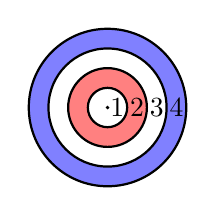
\begin{tikzpicture}[scale=0.25]
        % Outer circle (radius 4)
        \fill[blue!50] (0,0) circle (4);
        
        % Annular regions
        \fill[white] (0,0) circle (3);
        \fill[red!50] (0,0) circle (2);
        \fill[white] (0,0) circle (1);
        
        % Inner circle
        \fill[black] (0,0) circle (0.1); % A small black dot at the center
        
        % Draw the circle outlines
        \draw[thick] (0,0) circle (4);
        \draw[thick] (0,0) circle (3);
        \draw[thick] (0,0) circle (2);
        \draw[thick] (0,0) circle (1);
        
        % Labels
        \node at (3.5,0) {4}; % outermost region
        \node at (2.5,0) {3}; 
        \node at (1.5,0) {2}; 
        \node at (0.5,0) {1}; 
        
        
    \end{tikzpicture}
    \end{center}
 
\end{minipage}

\end{frame}




\end{document}
